%!TEX program = pdflatex
\documentclass{beamer}

\usepackage{etex}
\reserveinserts{28}

%\useoutertheme[glossy]{wuerzburg}
\useinnertheme[shadow,outline]{chamfered}
%\usecolortheme{shark}
\usecolortheme{beaver}
\beamertemplatenavigationsymbolsempty

\usefonttheme{professionalfonts}
\let\digamma\relax
\usepackage[scale=0.85,stdmathitalics=true,romanfamily=casual]{lucimatx}
\usefonttheme[stillsansseriftext]{serif}

\usepackage{bm}


\usepackage{fancyvrb}



\usepackage{textfit} % commands \scaletoheight{height}{text} and \scaletowidth{width}{text}

\usepackage{tikz}

\usepackage{tcolorbox}

\newtheorem{Alert}{Alert}
\newtheorem{Highlight}{Highlight}

\newcommand{\Species}[1]{{\rmfamily \itshape #1}}
\newcommand{\Real}{\ensuremath{\mathbb{R}}}
\newcommand{\RealN}{\ensuremath{\mathbb{R}^n}}
\newcommand{\RealP}{\ensuremath{\mathbb{R}^p}}
\newcommand{\Mtx}[1]{\ensuremath{\bm{#1}}}
\newcommand{\Inv}[1]{\ensuremath{#1^{-1}}}
\newcommand{\InvMtx}[1]{\ensuremath{\bm{#1}^{-1}}}
\newcommand{\Red}[1]{\textcolor{red}{#1}}
\newcommand{\PsInv}[1]{\ensuremath{\bm{#1}^{+}}}

\usepackage{booktabs}



% --- Macro \xvec
% From a tex.stackexchange.com answer by Todd Lehman
% http://tex.stackexchange.com/questions/44017/dot-notation-for-derivative-of-a-vector
\makeatletter
\newlength\xvec@height%
\newlength\xvec@depth%
\newlength\xvec@width%
\newcommand{\xvec}[2][]{%
  \ifmmode%
    \settoheight{\xvec@height}{$#2$}%
    \settodepth{\xvec@depth}{$#2$}%
    \settowidth{\xvec@width}{$#2$}%
  \else%
    \settoheight{\xvec@height}{#2}%
    \settodepth{\xvec@depth}{#2}%
    \settowidth{\xvec@width}{#2}%
  \fi%
  \def\xvec@arg{#1}%
  \def\xvec@dd{:}%
  \def\xvec@d{.}%
  \raisebox{.2ex}{\raisebox{\xvec@height}{\rlap{%
    \kern.05em%  (Because left edge of drawing is at .05em)
    \begin{tikzpicture}[scale=1]
    \pgfsetroundcap
    \draw (.05em,0)--(\xvec@width-.05em,0);
    \draw (\xvec@width-.05em,0)--(\xvec@width-.15em, .075em);
    \draw (\xvec@width-.05em,0)--(\xvec@width-.15em,-.075em);
    \ifx\xvec@arg\xvec@d%
      \fill(\xvec@width*.45,.5ex) circle (.5pt);%
    \else\ifx\xvec@arg\xvec@dd%
      \fill(\xvec@width*.30,.5ex) circle (.5pt);%
      \fill(\xvec@width*.65,.5ex) circle (.5pt);%
    \fi\fi%
    \end{tikzpicture}%
  }}}%
  #2%
}
\makeatother

% --- Override \vec with an invocation of \xvec.
\let\stdvec\vec
\renewcommand{\vec}[1]{\xvec[]{\bm{#1}}}
% --- Define \dvec and \ddvec for dotted and double-dotted vectors.
\newcommand{\dvec}[1]{\xvec[.]{#1}}
\newcommand{\ddvec}[1]{\xvec[:]{#1}}


\usepackage{pifont}
\newcommand{\weblink}{\ding{43}}  % hand with pointing finger

\definecolor{links}{HTML}{2A1B81}
\hypersetup{colorlinks,linkcolor=,urlcolor=magenta}

\usepackage{tikz}
\usepackage{caption}
\usepackage{subcaption}

\usepackage[inline]{asymptote}
\usepackage{marvosym} % for male/female symbols

\newcommand{\matindex}[1]{\scriptsize#1}% Matrix index
\usepackage{blkarray}



%===========================================================
% Title Info
\title{Scientific Computing for Biologists}
\subtitle{Principal Components Analysis and Eigenanalysis} % (optional)

\author{Paul M. Magwene}


\date{}

\begin{document}
%===========================================================
\begin{frame}
\titlepage
\end{frame}

%===========================================================
\begin{frame}
  \frametitle{Overview of Lecture}
  
\begin{itemize}
		\item Principal Components Analysis
		\begin{itemize}
			\item Variable space representation
			\item Subject space representation
			\item Mathematical constrains
			\item PC scores and loadings
			\item Dimension reduction			
		\end{itemize}		
		\item Eigenvectors and eigenvalues	
\end{itemize}

\end{frame}
%===========================================================


%===========================================================
\begin{frame}
  \frametitle{Least Squares Regression vs. Major Axis Regression}

\begin{center}
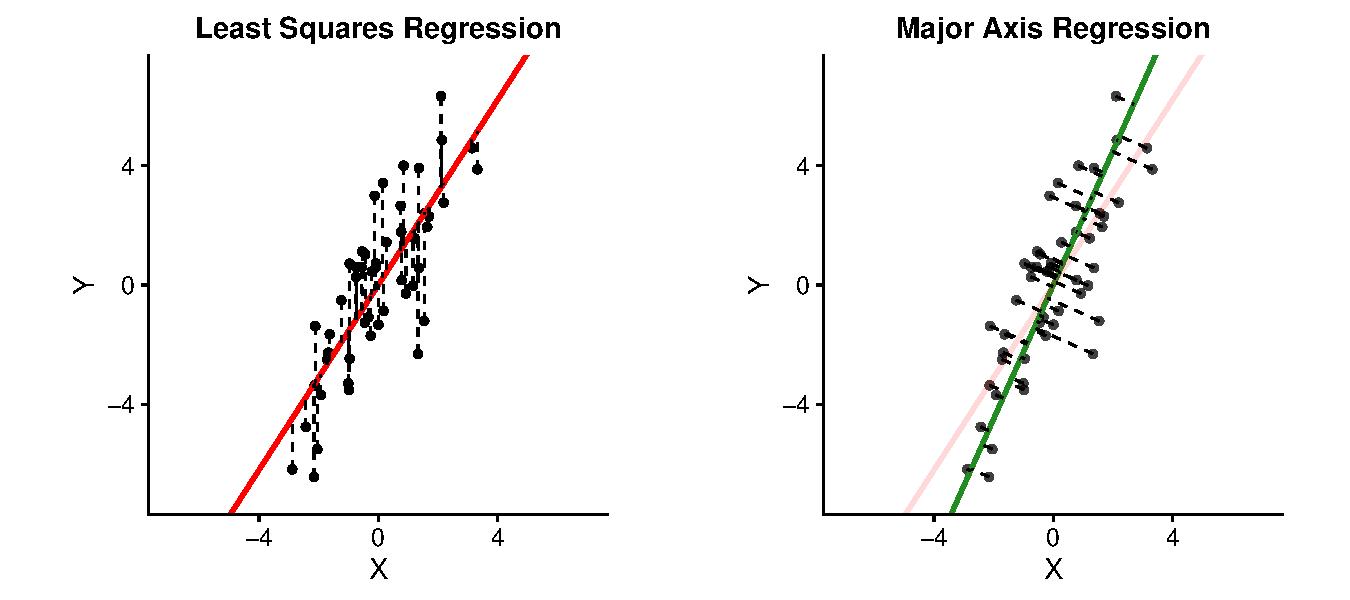
\includegraphics[width=\textwidth]{fig-lsqr-vs-major-axis.pdf}
\end{center}

\end{frame}
%===========================================================

%===========================================================
\begin{frame}
  \frametitle{Vector Geometry of Least Squares vs. Major Axis Regression}

\begin{figure}
\begin{center}
\subcaptionbox{OLS}{{\asyinclude[height=1.05in,keepAspect=true]{geom-OLS.asy}}}
\subcaptionbox{Major Axis Regression}{{\asyinclude[height=1.05in,keepAspect=true]{geom-majaxis.asy}}}
\end{center}
\caption{Vector geometry of ordinary least-squares and major axis regression.}
\end{figure}

\end{frame}
%===========================================================



% %===========================================================
% \begin{frame}
%   \frametitle{Example PC Basis}

% \begin{center}
% 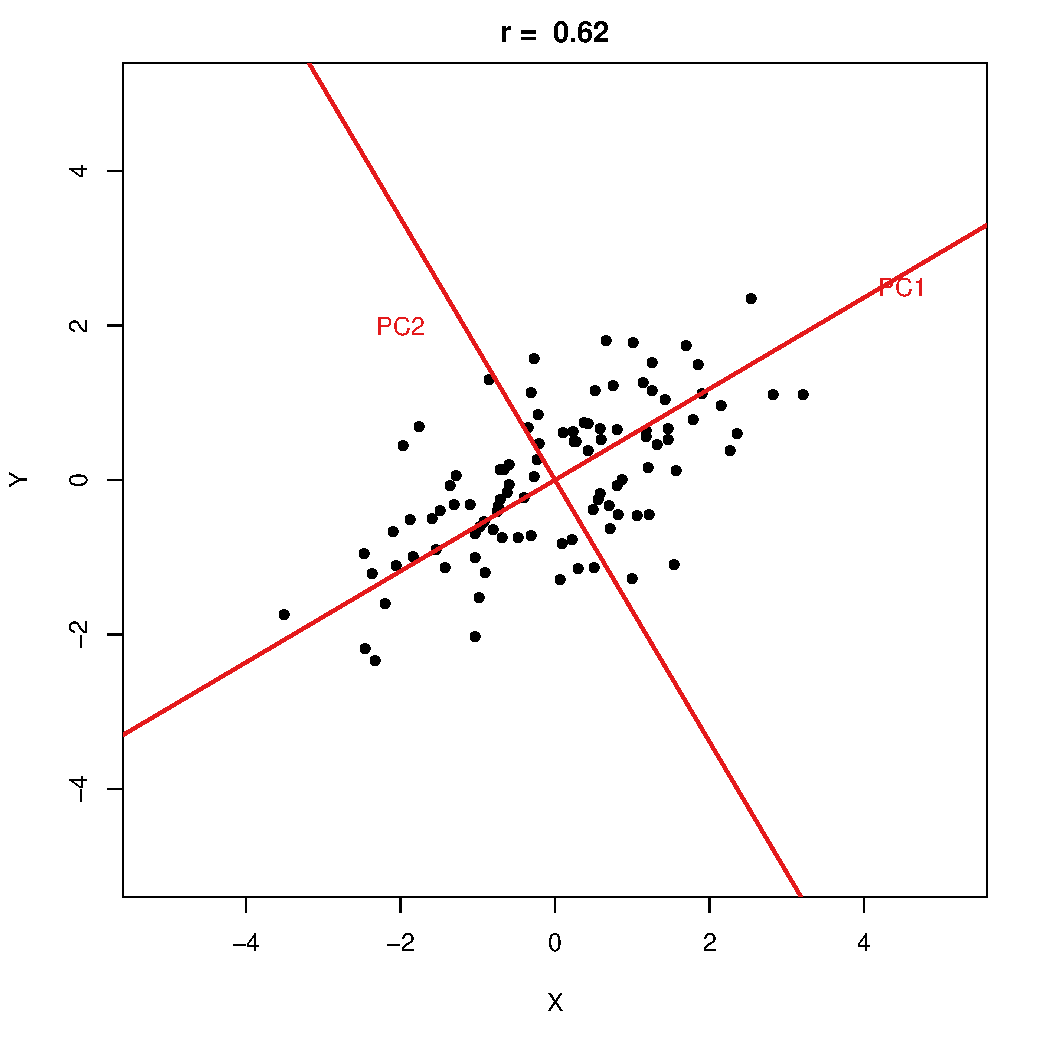
\includegraphics[height=2.75in]{fig-bivariate-pca.pdf}
% \smallskip

% Variable Space Representation

% \end{center}  


% \end{frame}
% %===========================================================

%===========================================================
\begin{frame}
  \frametitle{Contrast Between PC Axes and Regression}

\begin{center}
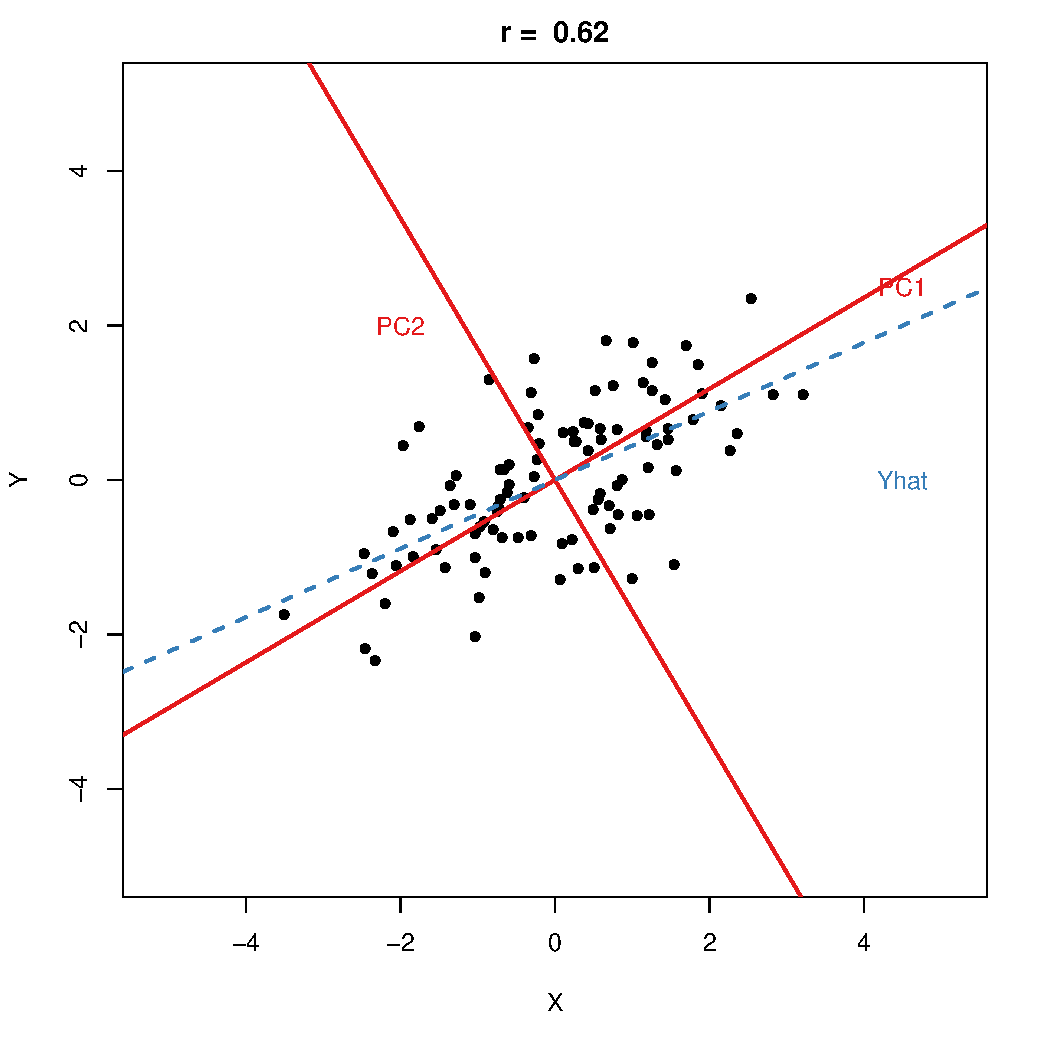
\includegraphics[height=2.75in]{fig-bivariate-pca-wreg.pdf}
\smallskip

\end{center}  

\end{frame}
%===========================================================

%===========================================================
\begin{frame}
  \frametitle{Observations with Respect to the PC Basis}

\begin{center}
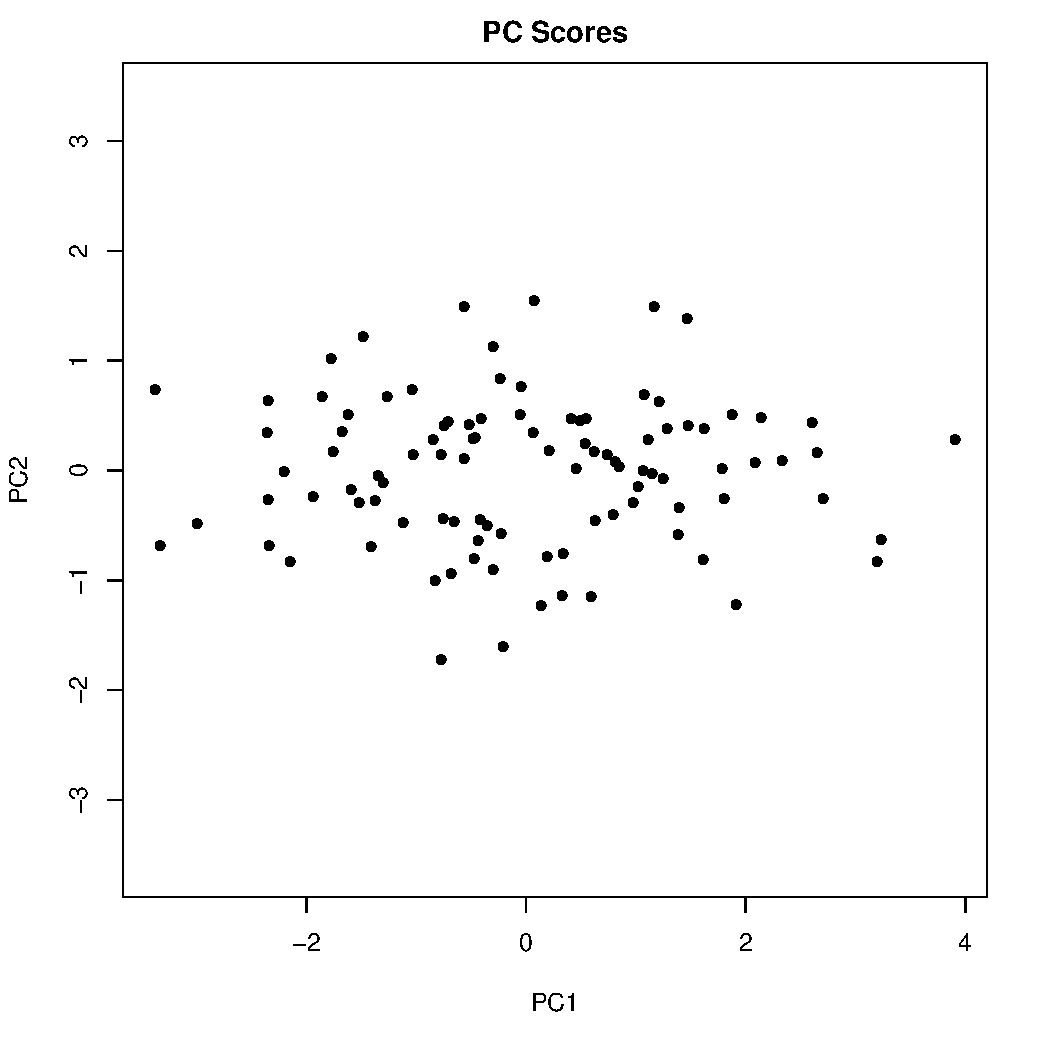
\includegraphics[height=2.75in]{fig-bivariate-pca-scores.pdf}
\smallskip

\end{center}  

\end{frame}
%===========================================================


%===========================================================
\begin{frame}
  \frametitle{Subject Space Representation of PCA}

\begin{center}
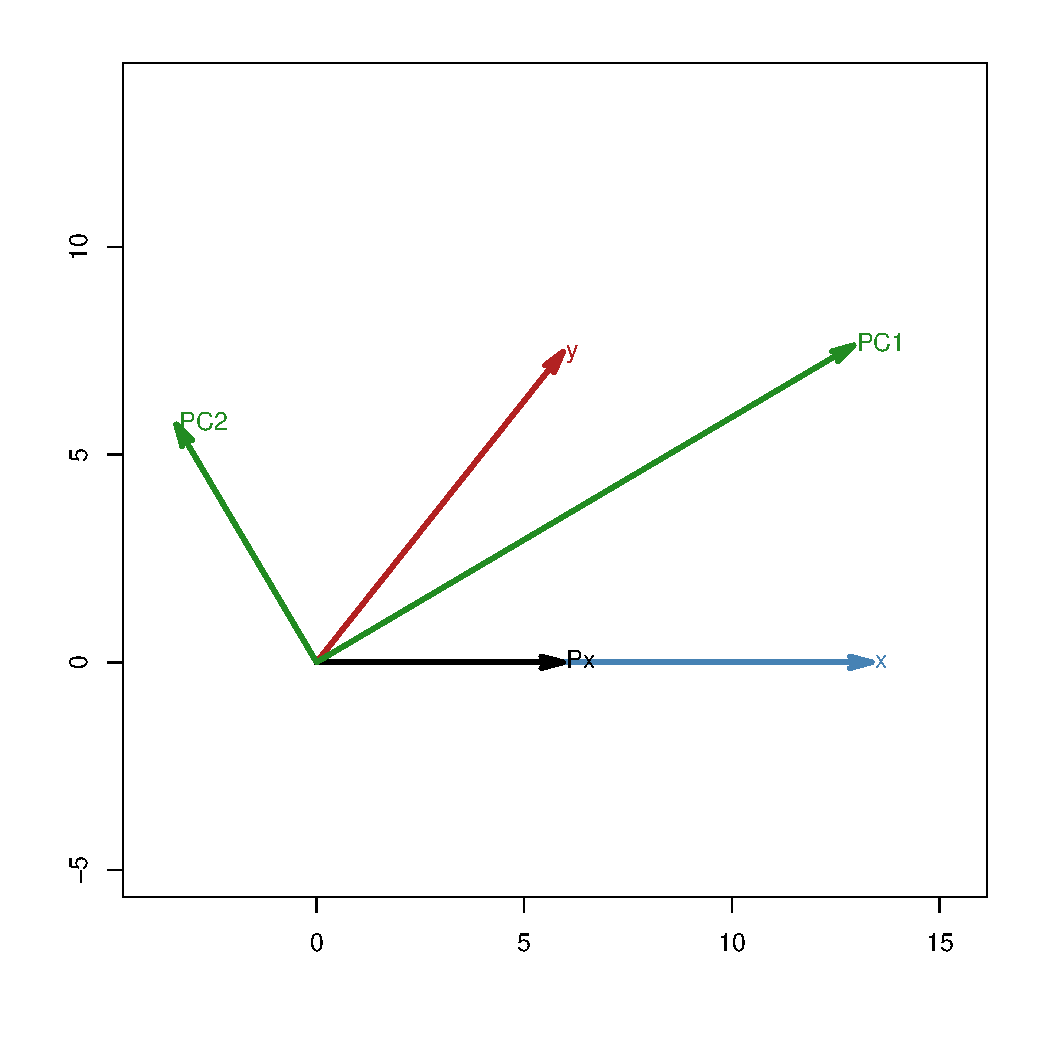
\includegraphics[height=2.5in]{fig-bivariate-pca-vectors.pdf}
\smallskip


\end{center}  

\end{frame}
%===========================================================




%===========================================================
\begin{frame}
  \frametitle{General Idea Behind PCA}


\begin{block}{Goal}

Define a new basis for describing your data that has ``nice'' properties.

\end{block}
\medskip

By nice we mean:
\begin{itemize}
    \item spans same space as original basis
    \item provides an orthogonal basis
    \item the order of the basis vectors is related to their relative ``importance"
    \item can be used to facilitate low dimensional summaries of high dimensional data
\end{itemize}


\end{frame}

%===========================================================


%===========================================================
\begin{frame}
  \frametitle{Space Spanned by a List of Vectors}


\begin{block}{Definition}

Let $X$ be a finite list of $n$-vectors. The \textbf{space spanned} by $X$ is the set of all vectors that can be written as linear combinations of the vectors in $X$.
\medskip

A space spanned includes the zero vector and is closed under addition and multiplication by a scalar.

\end{block}
\bigskip

Remember that a \emph{linear combination} of vectors is an equation of the form $z = b_1 \Mtx{x}_1 + b_2 \Mtx{x}_2 + \cdots + b_p \Mtx{x}_p$

\end{frame}

%===========================================================


%===========================================================
\begin{frame}
  \frametitle{Subspaces}

$\RealN$  denotes the seat of real $n$-vectors - the set of all $n \times 1$ matrices with entries from the set $\Real$ of real numbers.
\medskip

\begin{block}{Definition}

A \textbf{subspace} of $\Real^n$ is a subset S of $\Real^n$ with the following properties:
\begin{enumerate}
    \item $\Mtx{0} \in S$
    \item If $\Mtx{u} \in S$ then $k\Mtx{u} \in S$ for all real numbers $k$
    \item If $\Mtx{u} \in S$ and  $\Mtx{v} \in S$ then $\Mtx{u} + \Mtx{v} \in S$
\end{enumerate}

\end{block}

Examples of subspaces of $\Real^n$:
\begin{itemize}
    \item any space spanned by a list of vectors in $\Real^n$
    \item the set of all solutions to an equation $A\Mtx{x} = \Mtx{0}$ where $A$ is a $p \times n$ matrix, for any number p.
\end{itemize}

\end{frame}
%===========================================================

%===========================================================
\begin{frame}
  \frametitle{Basis}

Let $S$ be a subspace of \RealN.  Then there is a finite list, $X$, of vectors from $S$ such that $S$ is the space spanned by $X$.
\medskip

Let $S$ be a subspace of $\RealN$ spanned by the list $(u_1, u_2, \ldots, u_n)$. Then  there is a linearly independent sublist of $(u_1, u_2, \ldots, u_n)$ that also spans $S$.
\medskip

\begin{block}{Definition}
A list $X$ is a \textbf{basis} for $S$ if:
\begin{itemize}
\item $X$ is linearly independent
\item $S$ is the subspace spanned by $X$
\end{itemize}
\end{block}

\end{frame}
%===========================================================

%===========================================================
\begin{frame}
  \frametitle{Dimension}
Let $S$ be a subspace of \RealN.
\bigskip

\begin{block}{Definition}
The \textbf{dimension} of $S$ is the number of elements in a basis for $S$.
\end{block}

\end{frame}
%===========================================================






%===========================================================
\begin{frame}
  \frametitle{Mathematical Constraints on PCA}

The principal components are linear combinations of the original variables
\smallskip

\[ \begin{array}{ccc}
\vec{u}_1 & = & v_{11}\vec{x}_1 + v_{21}\vec{x}_2 + \cdots + v_{p1}\vec{x}_p \\
\vec{u}_2 & = & v_{12}\vec{x}_1 + v_{22}\vec{x}_2 + \cdots + v_{p2}\vec{x}_p \\
\vdots & & \vdots \\
\vec{u}_p & = & v_{1p}\vec{x}_1 + v_{2p}\vec{x}_2 + \cdots + v_{pp}\vec{x}_p \\
\end{array}
\]

\bigskip

In this formulation the $\vec{x}_i$ and $\vec{u}_i$ are column vectors.
\end{frame}
%===========================================================


%===========================================================
\begin{frame}
  \frametitle{Mathematical Constraints on PCA, cont.}



\begin{align*}
\underset{(n \times p)}{\Mtx{X}} &=  \begin{bmatrix}
x_{11} & x_{12} & \cdots & x_{1p}\\
x_{21} & x_{22} & \cdots & x_{2p}\\
\cdots & \cdots & \cdots & \cdots\\
x_{n1} & x_{p2} & \cdots & x_{np}\\
\end{bmatrix} & =  \begin{bmatrix}
\vec{x}_{1} & \vec{x}_{2} & \cdots & \vec{x}_{p}
\end{bmatrix} &  \\
\underset{(p \times p)}{\Mtx{V}}  &= \begin{bmatrix}
v_{11} & v_{12} & \cdots & v_{1p}\\
v_{21} & v_{22} & \cdots & v_{2p}\\
\cdots & \cdots & \cdots & \cdots\\
v_{p1} & v_{p2} & \cdots & v_{pp}\\
\end{bmatrix} & = \begin{bmatrix}
\vec{v}_{1} & \vec{v}_{2} & \cdots & \vec{v}_{p}
\end{bmatrix} & \\
\underset{(n \times p)}{\Mtx{U}}  &= \begin{bmatrix}
u_{11} & u_{12} & \cdots & u_{1p}\\
u_{21} & u_{22} & \cdots & u_{2p}\\
\cdots & \cdots & \cdots & \cdots\\
u_{n1} & u_{p2} & \cdots & u_{np}\\
\end{bmatrix} &= \begin{bmatrix}
\vec{u}_{1} & \vec{u}_{2} & \cdots & \vec{u}_{p}
\end{bmatrix} &= \Mtx{X}\Mtx{V}
\end{align*}



\end{frame}
%===========================================================

%===========================================================
\begin{frame}
  \frametitle{Mathematical Constraints on PCA, cont.}

\begin{itemize}
  \item The PCs are orthogonal:
\[
\vec{u}_j \cdot \vec{u}_k = 0 \mbox{ for all } j \neq k.
\]


	\item The sum of the squared coefficients for each PC is fixed to unity:
\[
\vec{v}_k \cdot \vec{v}_k = 1
\]

	\item The sum of the squared lengths for the original variables and the PCs is the same:
\[
|\vec{x}_1|^2 + |\vec{x}_2|^2 + \cdots + |\vec{x}_p|^2 = |\vec{u}_1|^2 + |\vec{u}_2|^2 + \cdots + |\vec{u}_p|^2
\]	


	\item The PCs are ordered such that:

\[
 |\vec{u}_1|^2 \geq |\vec{u}_2|^2  \geq \cdots \geq |\vec{u}_p|^2
\]

\end{itemize}

\end{frame}

%===========================================================


%===========================================================
\begin{frame}
  \frametitle{Principal Component Scores}

\begin{block}{Definition}
The PC scores are the components of the original observations with respect to the principal components (i.e. the observations projected into the new basis).
\end{block}
\medskip

If the values of the $i$-th individual in the original variables are:
\[
\begin{array}{cccccc}
\Mtx{r}_i & = & [x_{i1}, & x_{i2}, & \cdots & x_{ip}]
\end{array}
\]

then the score of that individual on the $k$-th principal component axis is given by:

\[
\Mtx{U}_{ik} = \Mtx{r}_i \cdot \Mtx{v}_k = v_{1k}x_{i1} + v_{2k}x_{i2} + \cdots + v_{pk}x_{ip}
\]

\end{frame}
%===========================================================


%===========================================================
\begin{frame}
  \frametitle{Principal Component Loadings}

The \textbf{loading vector} of the $k$-th PC is:

\[
|\Mtx{u}_k|\Mtx{v}_k
\]

The \textbf{loading} of the $j$-th original variable on the $k$-th PC is:

\[
|\Mtx{u}_k|v_{jk}
\]

\begin{block}{Interpretation}
Loadings give a sense of the relative contribution of each of the original variables to the PCs.

\begin{itemize}
    \item When the input data is unscaled, loadings are the covariances between the original variables and the PCs
    \item When the input data are scaled (i.e. sd = 1), loading are the correlations between the original variables and the PCs
\end{itemize}

\end{block}

\end{frame}
%===========================================================

%===========================================================
\begin{frame}[fragile]
  \frametitle{PCA Example: Jolicoeur and Mosimann's Turtle Data Set}

\begin{center}
\hspace*{-0.8cm}
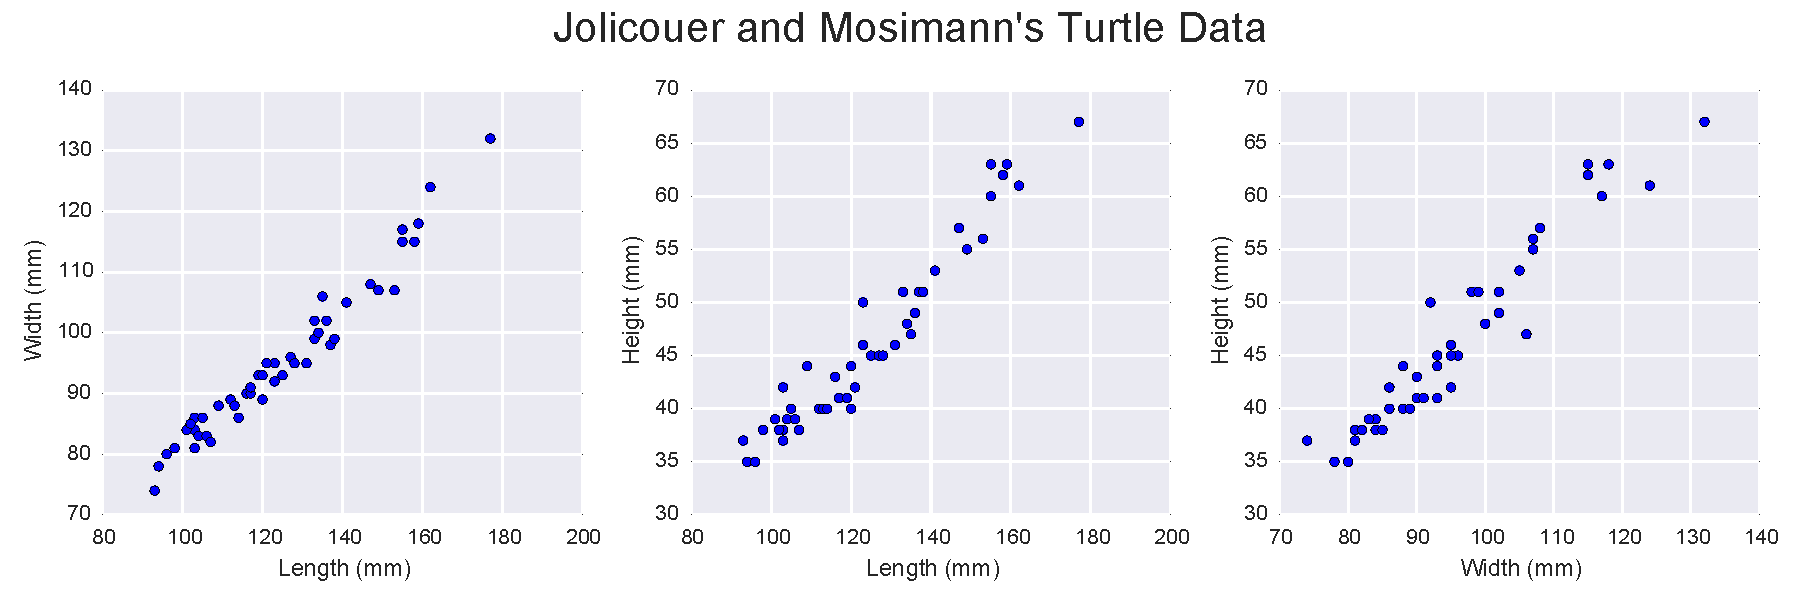
\includegraphics[width=0.95\paperwidth]{turtles.pdf}
\end{center}
\end{frame}

%===========================================================

%===========================================================
\begin{frame}
  \frametitle{PCA Example: Jolicoeur and Mosimann's Turtle Data Set}

\begin{itemize}
\item 48 specimens (\Male,\Female), 3 variables (length, width, height)

\item Covariance and correlation matrices:
\footnotesize{
\[
\mathsf{cov}(\Mtx{X}) = \left[ \begin{array}{rrr}
420 & 254 & 165 \\
       & 161 & 102 \\
       &        &   70\\
\end{array}
\right]
\;
;
\;
\mathsf{cor}(\Mtx{X}) = \left[ \begin{array}{ccc}
1 & 0.978 & 0.964 \\
       & 1 & 0.961\\
       &        &   1\\
\end{array}
\right]
\]
} % end \small

\item Principal components (using correlation matrix), proportion of variance:

{\small
\begin{center}
\begin{tabular}{ccc}
PC1 & PC2 & PC3 \\ \hline
0.978 & 0.014 & 0.007
\end{tabular}
\end{center}
} % end \small

\item Principal component loadings:

{\small
\begin{center}
\begin{tabular}{lccc}
&PC1 & PC2 & PC3 \\ \cline{2-4}
L & 0.579 & -0.325 & 0.748 \\
W & 0.578 & -0.483 & -0.657 \\
H & 0.575 & 0.813 &  0.092 \\
\end{tabular}
\end{center}
} % end \small



\end{itemize}


\end{frame}

%===========================================================
\begin{frame}
  \frametitle{Turtle PCA Plots}

\begin{center}
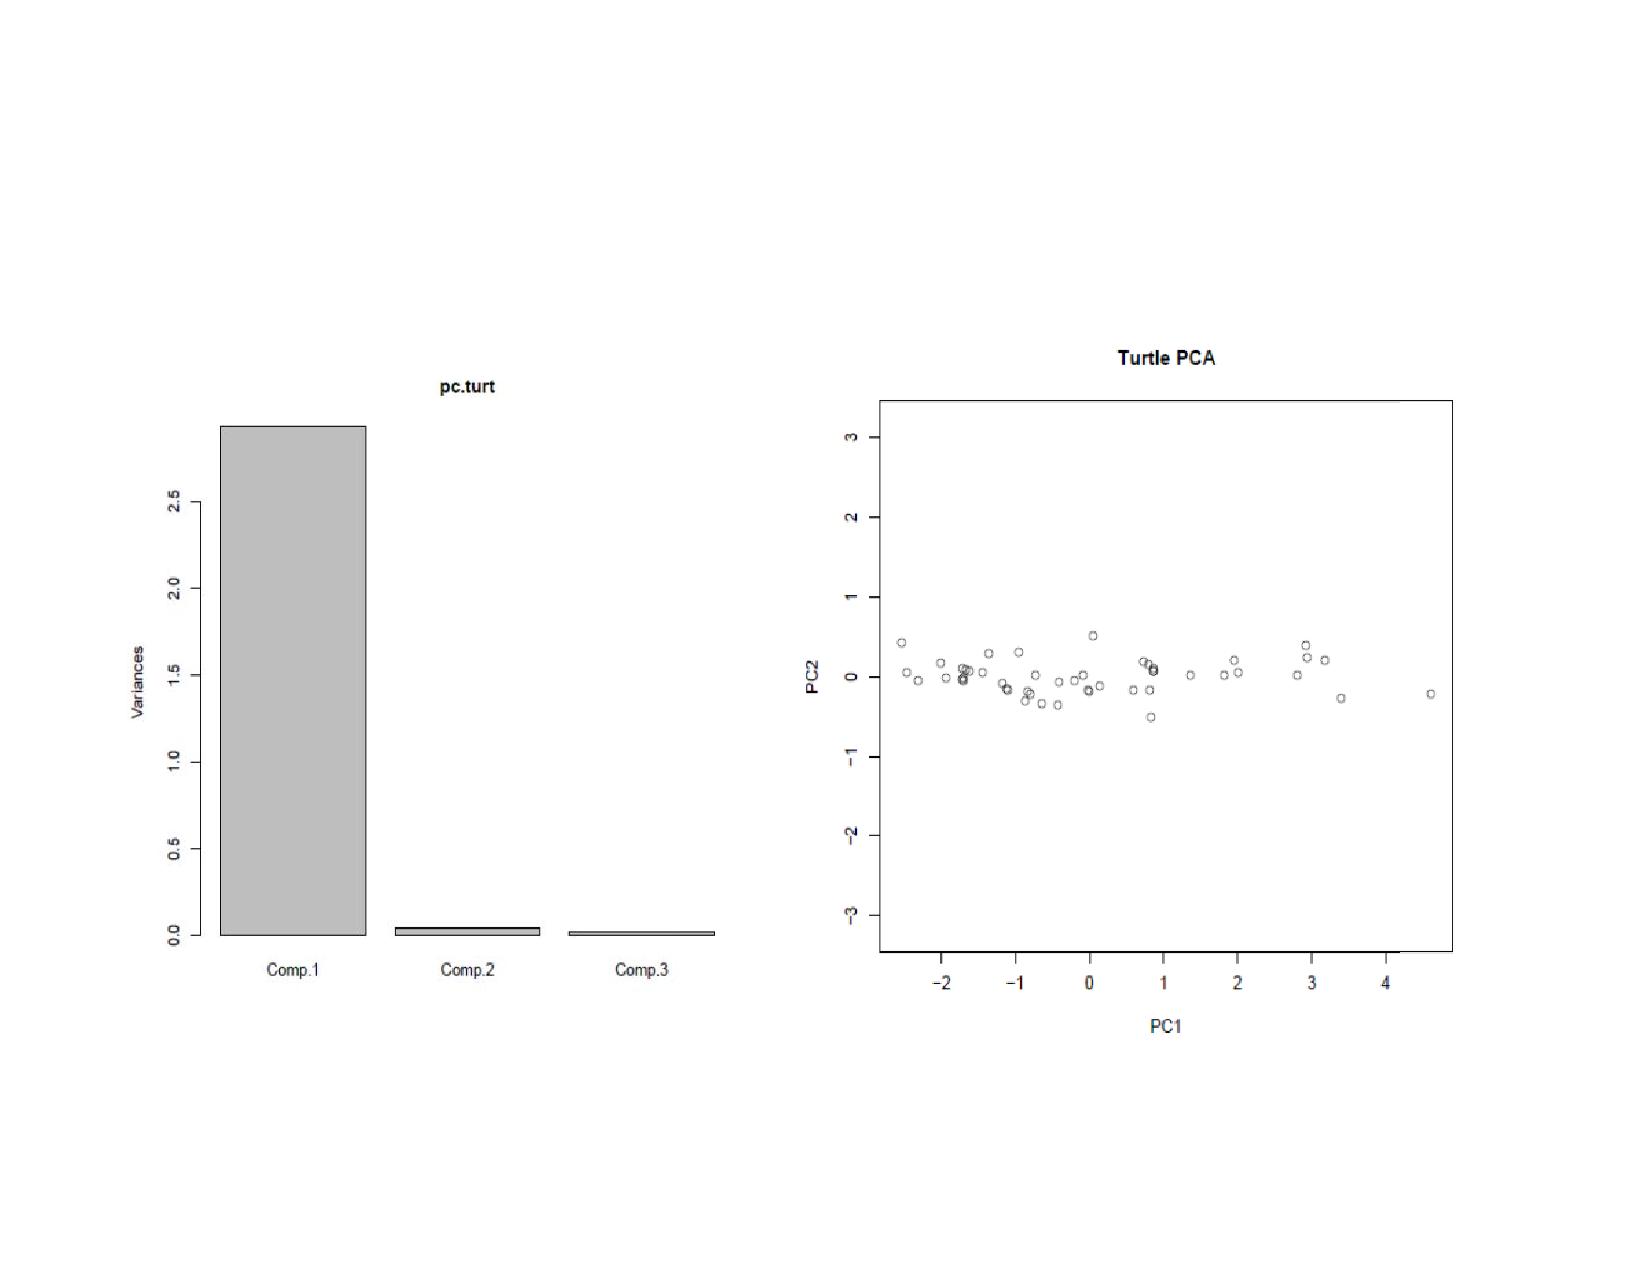
\includegraphics[height=2in]{turtle-pca.pdf}
\end{center}
\end{frame}

%===========================================================

% %===========================================================
% \begin{frame}[fragile]
%   \frametitle{Bivariate Example Revisited}

% \begin{columns}[c]
  
% \column{0.5\textwidth}
% \begin{Rcode}
% > cov(z)
%          [,1]      [,2]
% [1,] 1.865551 0.6523660
% [2,] 0.652366 0.9248509

% > z.pca
% Standard deviations:
% [1] 1.4830530 0.7687363

% Rotation:
%             PC1        PC2
% [1,] -0.8901780 -0.4556128
% [2,] -0.4556128  0.8901780

% > A <- z.pca$rotation # coefficients
% > L <- diag(z.pca$sdev) # lengths of PCs
% > A %*% L  # loadings
%           [,1]       [,2]
% [1,] -1.320181 -0.3502461
% [2,] -0.675698  0.6843122
% \end{Rcode}

% \column{0.5\textwidth}
% \begin{Rcode}
% > (A %*% L)**2  # loadings squared
%           [,1]      [,2]
% [1,] 1.7428784 0.1226723
% [2,] 0.4565677 0.4682832
% > apply(z, 2, var) # variance of orig.
% [1] 1.8655507 0.9248509
% \end{Rcode}
% 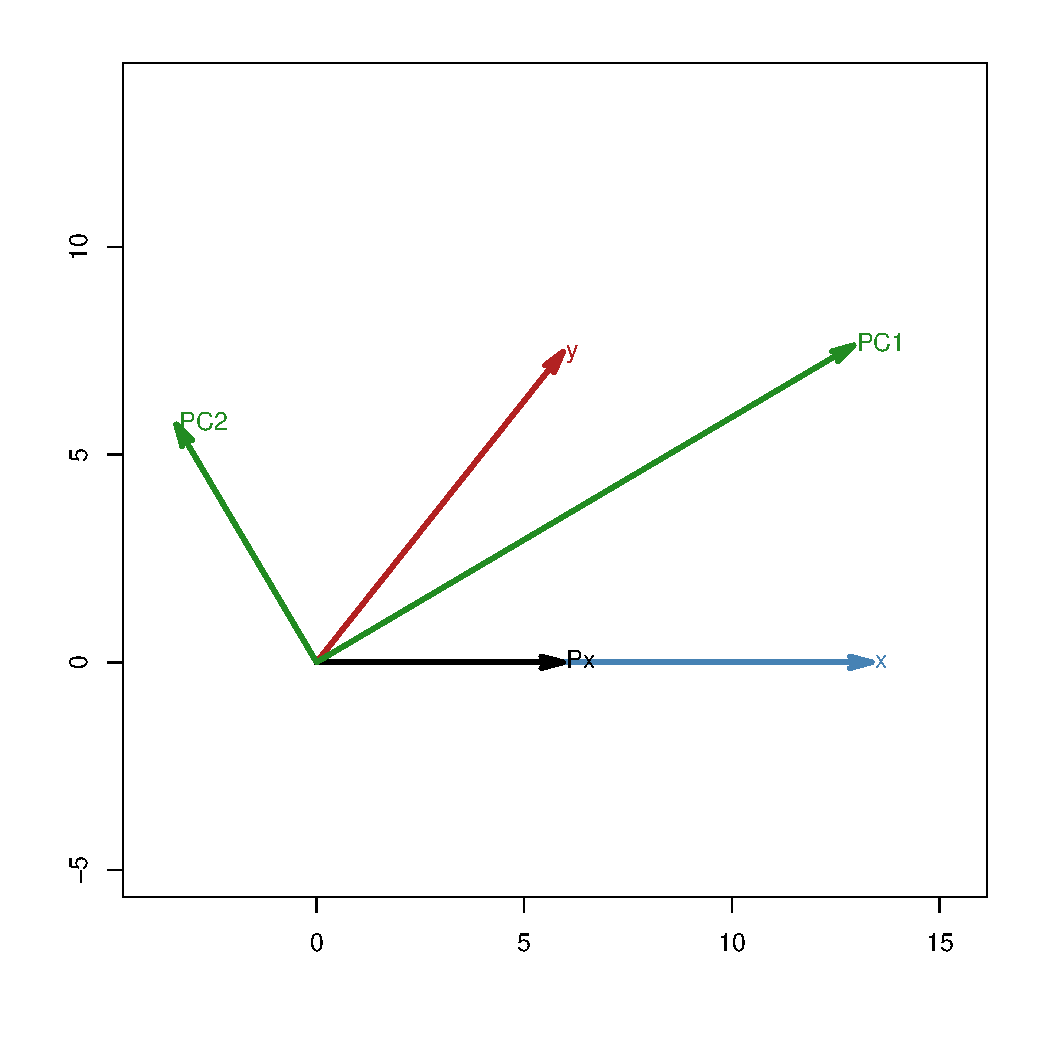
\includegraphics[width=\textwidth]{fig-bivariate-pca-vectors.pdf}

% \end{columns}

% \end{frame}
% %===========================================================



%===========================================================
\begin{frame}
  \frametitle{PCA Cautions and Caveats}

\begin{description}

\item[Scale matters] \mbox{}\\
If the original variables are not measured on comparable scales they should be standardized prior to PCA

\item[PCA emphasizes correlated variables] \mbox{}\\
If one of the original variables is (nearly) independent of the other variables than it will have weak loadings on the major PCs. But this doesn't mean it's unimportant!

\item[PCA does not represent a model] \mbox{}\\
It's simply a transformation of the original data.

\end{description}

\end{frame}

%===========================================================
\begin{frame}
  \frametitle{PCA for Dimension Reduction}


A common application of PCA is to find a lower dimensional representation of a high dimensional data set.
\bigskip 

\begin{block}{Goal}
Capture the majority of the variance with just a few principal component axes.
\end{block}

\end{frame}

%===========================================================





%===========================================================
\begin{frame}
  \frametitle{}

\begin{center}
\begin{Huge}
Eigenvectors and Eigenvalues
\end{Huge}
\end{center}
\end{frame}

%===========================================================


%===========================================================
\begin{frame}
  \frametitle{Matrices as Linear Transformations}

\begin{itemize}  

\item Let $A$ be a particular $n \times p$ matrix. Than for any $p$-vector \Mtx{x}, the product $A\Mtx{x}$ is a $n$-vector.

\item We say that the matrix $A$ determines a function from $\Real^p$ to $\Real^n$.  

\begin{itemize}
\item $A(k \Mtx{x}) = k(A \Mtx{x})$ where $k$ is a scalar.
\item If \Mtx{y} is also a $p$-vector than $A(\Mtx{x}+\Mtx{y}) = A\Mtx{x} + A\Mtx{y}$ is  an $n$-vector
\end{itemize}


\item A function, $\mathit{f}$, where $\mathit{f}(\Mtx{x} + \Mtx{y}) = \mathit{f}(\Mtx{x}) + \mathit{f}(\Mtx{y})$ and $\mathit{f}(k\Mtx{x}) = k\mathit{f}(\Mtx{x})$ is called a \emph{\textbf{linear transformation}}.

\end{itemize}

\begin{Highlight}
Every matrix determines a linear transformation!

\medskip

Every linear transformation can be represented by a matrix!
\end{Highlight}

\end{frame}
%===========================================================


%===========================================================
\begin{frame}[fragile]
  \frametitle{Examples of Linear Transformation in $\Real^2$}


\begin{itemize}
\item reflection in the $x$-axis

\[
\left[
\begin{array}{cc}
1 & 0 \\
0 & -1  
\end{array}
\right]:
\left[
\begin{array}{c}
x \\ y 
\end{array}
\right]
\mapsto
\left[
\begin{array}{c}
x \\ -y 
\end{array}
\right]
\]

\item reflection in the line $y = x$

\[
\left[
\begin{array}{cc}
0 & 1 \\
1 & 0  
\end{array}
\right]:
\left[
\begin{array}{c}
x \\ y 
\end{array}
\right]
\mapsto
\left[
\begin{array}{c}
y \\ x 
\end{array}
\right]
\]

\item shear parallel to the $x$-axis
\[
\left[
\begin{array}{cc}
1 & a \\
0 & 1  
\end{array}
\right]:
\left[
\begin{array}{c}
x \\ y 
\end{array}
\right]
\mapsto
\left[
\begin{array}{c}
x+ay \\ y 
\end{array}
\right]
\]

\item projection onto the $x$-axis
\[
\left[
\begin{array}{cc}
1 & 0 \\
0 & 0  
\end{array}
\right]:
\left[
\begin{array}{c}
x \\ y 
\end{array}
\right]
\mapsto
\left[
\begin{array}{c}
x \\ 0 
\end{array}
\right]
\]


\item How about reflection in the $y$-axis? shear parallel to the $y$-axis? projection onto the $y$-axis?

\end{itemize}

\end{frame}
%===========================================================

%===========================================================
\begin{frame}
  \frametitle{Examples of Linear Transformation: Rotation}


\begin{itemize}
\item The rotation of the plane, by an angle $\theta$ about the origin is given by:
\[
A = \left[
\begin{array}{cc}
\cos \theta & -\sin \theta\\ 
\sin \theta & \cos \theta 
\end{array}
\right]
\]
\end{itemize}

\begin{center}

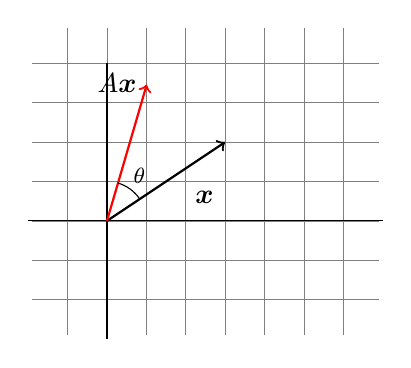
\begin{tikzpicture}[x=0.5cm, y=0.5cm]

\draw[step=0.5cm, style=help lines] (-1.9,-2.9) grid (6.9,4.9);
\draw (-2,0) -- (7,0);
\draw (0,-3) -- (0,4);

\draw[thick,->] (0,0) -- (3,2);
\draw (2,1) node[below right] {\Mtx{x}};

\draw[thick,red,->] (0,0) -- (1.01,3.46);
\draw (1,3) node[above left] {$A\Mtx{x}$};

\draw (0,0) +(34:0.5cm) arc (34:74:0.5cm);
\path (0,0) ++(54:0.7cm) node[font=\footnotesize] {$\theta$};

%\draw (1.5,1) arc (34:74:1cm);
%\path (0,0) ++(55:1.1cm) node[font=\footnotesize] {$\theta$};

\end{tikzpicture}

\end{center}


\end{frame}
%===========================================================




%===========================================================
\begin{frame}
  \frametitle{Linear Transformations and Eigenvectors/Eigenvalues}

If $\Mtx{A}$ is a $p \times p$ matrix, then:

\begin{itemize}
\item The \textbf{eigenvectors} of $\Mtx{A}$ represent directions in $\RealP$ that are unchanged by the transformation represented by $\Mtx{A}$

\item Vectors along the directions defined by the eigenvectors may be scaled however. The relative scaling is given by the \textbf{eigenvalues} of $\Mtx{A}$

\end{itemize}
\medskip

if $\Mtx{A}\Mtx{v} = k\Mtx{v}$ for some scalar $k$ than:
\begin{itemize}
\item  $\Mtx{v}$ is an eigenvector of $\Mtx{A}$ 
\item $k$ is it's associated eigenvalue.
\end{itemize}

\end{frame}
%===========================================================
\begin{frame}
  \frametitle{Example Linear Transformation}

\begin{center}
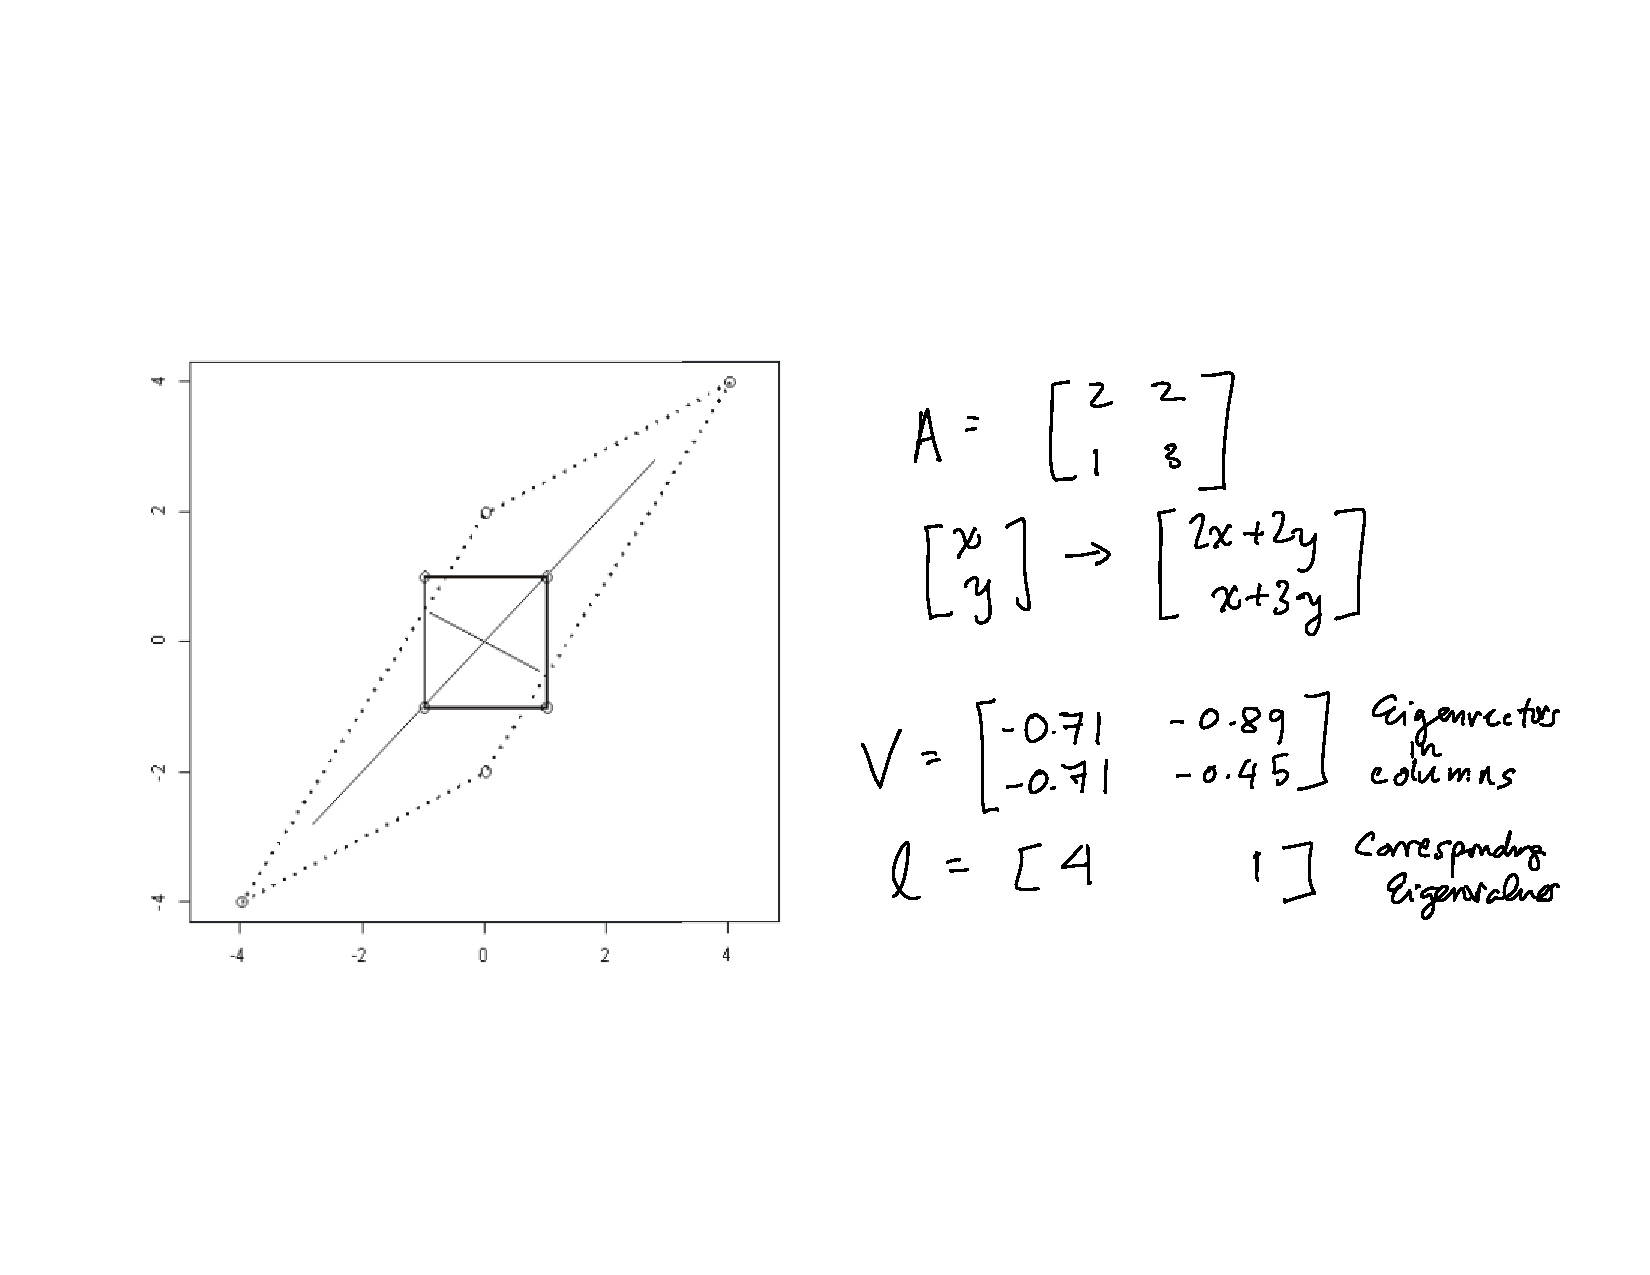
\includegraphics[height=2in]{eigen-example.pdf}
\medskip

Note that the eigenvectors above are \emph{not} orthogonal.

\end{center}  

\end{frame}
%===========================================================
\begin{frame}
  \frametitle{More on Eigenvectors and Eigenvalues}

\begin{itemize}
 	\item Eigenvectors/eigenvalues are only defined for square matrices
	\item Eigenvectors are not, in general, orthogonal
\end{itemize}
\smallskip

However, if $\Mtx{A}$ is a real symmetric matrix then:
\begin{itemize}
	\item eigenvectors of $\Mtx{A}$ are guaranteed to be orthogonal
	\item eigenvalues of $\Mtx{A}$ are guaranteed to be real
	\item $\Mtx{A}$ has zero-valued eigenvectors \emph{iff} $\Mtx{A}$ is singular
	\item if $\Mtx{V}$ is the matrix of eigenvectors we can write:
\[
	\Inv{\Mtx{V}} \Mtx{A} \Mtx{V} = \Mtx{D}
\]
where $\Mtx{D}$ is a diagonal matrix with eigenvalues on the diagonal:
\footnotesize{
\[\Mtx{D} = 
 \left[ \begin{array}{rrr}
l_1 &  & 0 \\
       & l_2 & \\
 0      &        &  l_3\\
\end{array}
\right]
\]
} % end \footnotesize

\end{itemize}



\end{frame}
%===========================================================



%===========================================================
\begin{frame}[fragile]
  \frametitle{Calculation of PCs}

Principal components can be calculated by eigenanalysis of the covariance or correlation matrix.
%
\begin{align*}
\underset{(n \times p)}{\Mtx{X}} & =  
\begin{bmatrix}
\vec{X}_{1} & \vec{X}_{2} & \cdots & \vec{X}_{p}
\end{bmatrix} &   
\text{Data matrix w/variables in columns}  \\
%
\underset{(p \times p)}{\Mtx{S}}  &= 
\cov(X) & \text{Covariance or correlation matrix of X}  \\
%
\underset{(p \times p)}{\Mtx{V}}  &= 
\begin{bmatrix}
\vec{v}_{1} & \vec{v}_{2} & \cdots & \vec{v}_{p}
\end{bmatrix} & 
\text{Matrix of eigenvectors of S} \\
%
\underset{(1 \times p)}{\Mtx{l}}  &= 
\begin{bmatrix}
l_{1} & l_{2} & \cdots & l_{p}
\end{bmatrix} & 
\text{Vector of eigenvalues of S}
\end{align*}

Given the above:

\begin{itemize}
  \item PC scores matrix: $\underset{(p \times p)}{\Mtx{U}} = \Mtx{X}\Mtx{V}$

  \item PC loadings matrix:  $\Mtx{V}\Mtx{L}^{1/2}$ where $\Mtx{L}^{1/2} = %
\begin{bsmallmatrix}
\sqrt{l_1} &  & \text{\Large 0} \\
 & \ddots & \\
\text{\Large 0} &  & \sqrt{l_p} \\
\end{bsmallmatrix}
$

  \item Variance summarized by k-th PC: $\sqrt{l_k}$
\end{itemize}



\end{frame}
%===========================================================


\end{document}


%===========================================================
\begin{frame}
  \frametitle{XXX}

\end{frame}
%===========================================================
